%% start of file `template.tex'.
%% 
%% Original Copyright 2006-2013 Xavier Danaux (xdanaux@gmail.com).
%% Modified Copyright 2021-2022: Rajib Das Bhagat (rajibdasbhagat@gmail.com).
%
% This work may be distributed and/or modified under the
% conditions of the LaTeX Project Public License version 1.3c,
% available at http://www.latex-project.org/lppl/.


\documentclass[11pt,a4paper,sans]{moderncv}        % possible options include font size ('10pt', '11pt' and '12pt'), paper size ('a4paper', 'letterpaper', 'a5paper', 'legalpaper', 'executivepaper' and 'landscape') and font family ('sans' and 'roman')

\usepackage[utf8]{vietnam}

% moderncv themes
\moderncvstyle{banking}                            % style options are 'casual' (default), 'classic', 'oldstylef' and 'banking'
\moderncvcolor{black}                                % color options 'blue' (default), 'orange', 'green', 'red', 'purple', 'grey' and 'black'
%\renewcommand{\familydefault}{\sfdefault}         % to set the default font; use '\sfdefault' for the default sans serif font, '\rmdefault' for the default roman one, or any tex font name
%\nopagenumbers{}                                  % uncomment to suppress automatic page numbering for CVs longer than one page

% character encoding
\usepackage[utf8]{inputenc}                       % if you are not using xelatex ou lualatex, replace by the encoding you are using
%\usepackage{CJKutf8}                              % if you need to use CJK to typeset your resume in Chinese, Japanese or Korean
\usepackage{fontawesome}
\usepackage{comment}
% adjust the page margins
\usepackage[scale=0.9]{geometry}
%\setlength{\hintscolumnwidth}{3cm}                % if you want to change the width of the column with the dates
%\setlength{\makecvtitlenamewidth}{10cm}           % for the 'classic' style, if you want to force the width allocated to your name and avoid line breaks. be careful though, the length is normally calculated to avoid any overlap with your personal info; use this at your own typographical risks...


% personal data
\name{Nguyễn Văn Lộc}{(Nguyen Van Loc)}
\title{Student}
\insti{University of Science, Vietnam National University Ho Chi Minh City}
%\extrainfo{Placement Registration Number: Y/33/CS/20/067}
\address{Place: VNUHCM Dorm B}{Thu Duc}{Ho Chi Minh City, Vietnam}
% optional, remove / comment the line if not wanted; the "postcode city" and and "country" arguments can be omitted or provided empty
\phone[mobile]{+84-905481342}                   % optional, remove / comment the line if not wanted
%\phone[fixed]{+2~(345)~678~901}                    % optional, remove / comment the line if not wanted
%\phone[fax]{+3~(456)~789~012}                      % optional, remove / comment the line if not wanted
\email{vanloc1808@gmail.com}                               % optional, remove / comment the line if not wanted
\homepage{linkedin.com/in/vanloc1808/}                         % optional, remove / comment the line if not wanted

\extrainfo{\homepagesymbol \httplink{github.com/vanloc1808}}
                % optional, remove / comment the line if not wanted
% \photo[64pt][0.4pt]{logo.png}                       % optional, remove / comment the line if not wanted; '64pt' is the height the picture must be resized to, 0.4pt is the thickness of the frame around it (put it to 0pt for no frame) and 'picture' is the name of the picture file
%\quote{Love thy journey, never thy destination!}                           
%----------------------------------------------------------------------------------
%            content
%----------------------------------------------------------------------------------
\begin{document}
%\begin{CJK*}{UTF8}{gbsn}                          % to typeset your resume in Chinese using CJK
%-----       resume       ---------------------------------------------------------
%\makecvtitle
\hypersetup{
    linkcolor=blue,
    filecolor=magenta,      
    urlcolor=cyan,
}
\urlstyle{same}

\noindent
\begin{minipage}{.78\textwidth}
 \makecvtitle
\end{minipage}%
\begin{minipage}{.30\textwidth}
  \centering
  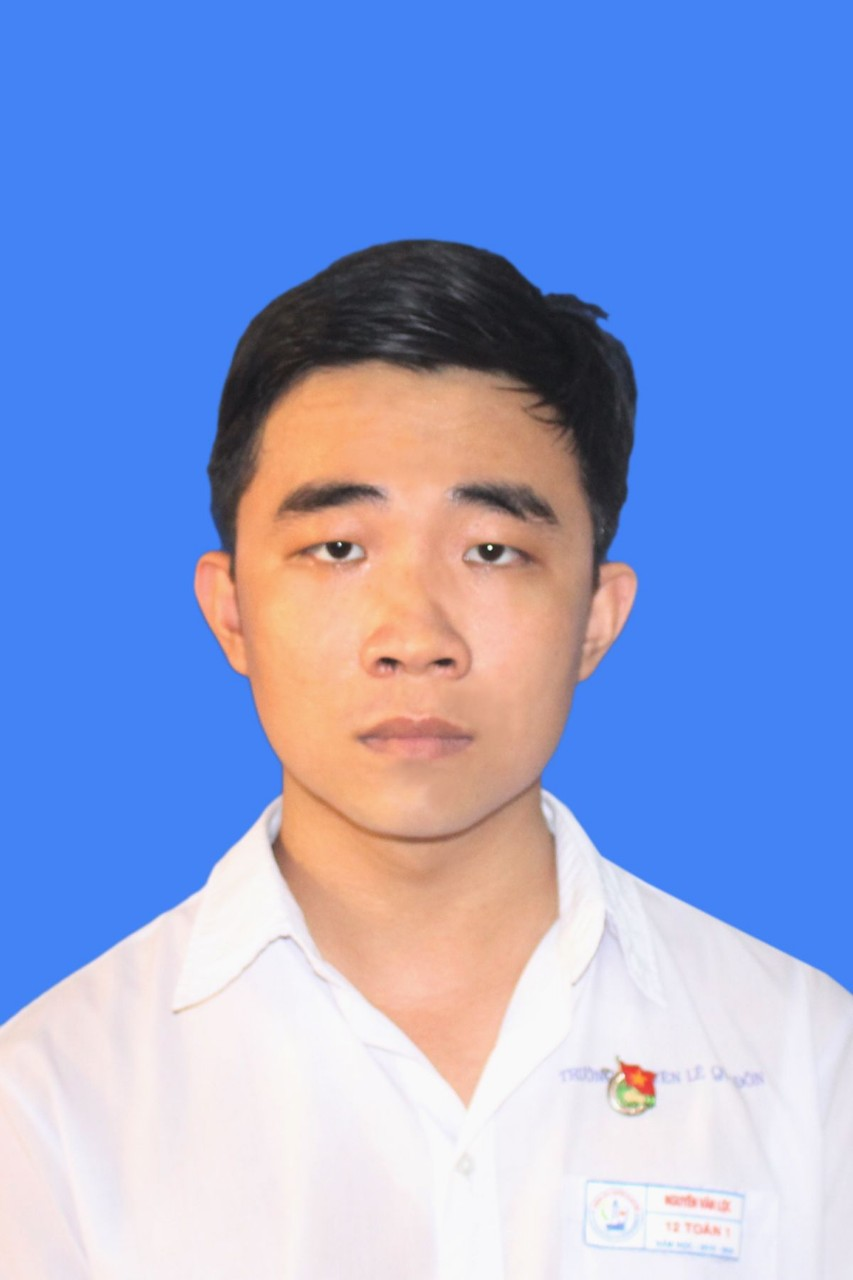
\includegraphics[height=3cm]{avt.jpg}
\end{minipage}
\vspace{-1em}
\section{Applications for}
\begin{itemize}
\item Data Science Intern
\item Data Engineer Intern
\item AI Engineer Intern
\end{itemize}
\vspace{-1em}
\input{src/education}
\vspace{-1em}

\section{Knowledge}
\cvlistdoubleitem{Data Structures and Algorithms}{Databases}
\cvlistdoubleitem{Computer Networks}{Combinatorics}
\cvlistdoubleitem{Probability and Statistics}{Linear Algebra}
\cvlistdoubleitem{Exploratory Data Analysis}{Data Visualization}
\cvlistdoubleitem{Machine Learning}{}

\vspace{-1em}

\section{Technical Skills}
\cvlistitem{Programming Techniques}
\cvlistitem{Object-Oriented Programming}
\cvlistitem{Socket Programming}
\cvlistitem{Programming Languages: C, C++, Python, R}
\cvlistitem{Web Technologies: HTML, CSS, JavaScript (basic)}
\cvlistitem{Database System: Microsoft SQL Server}
\cvlistitem{Operating Systems: Windows, Linux (Ubuntu, Kubuntu)}
\cvlistitem{Jupyter Notebook}
\cvlistitem{Git and GitHub}
\cvlistitem{{Tools:} {\LaTeX, Anaconda, Microsoft Office}}
\vspace{-1em}

%\input{src/key_projects}
%\vspace{-1em}

\input{src/course_projects}
\vspace{-1em}
\section{Online Courses }
\cvlistitem {Coursera: \\ 
\textit{\href{https://www.coursera.org/account/accomplishments/professional-cert/VA25F52RCVC9}{\textcolor{blue}{IBM Data Science Professional Certificate}}} (August 2022),\\
\textit{\href{https://www.coursera.org/account/accomplishments/verify/CLD23RCC4TXN}{\textcolor{blue}{Writing in the Sciences}}} (September 2021)
}

% \cvlistitem {Jovian: \\ 
%\textit{\href{cert link}{\textcolor{blue}{course name}}} (time),\\
%\textit{\href{cert link}{\textcolor{blue}{course name}}} (time),\\
%\textit{\href{cert link}{\textcolor{blue}{course name}}} (time)\\
%}

\vspace{-1em}

\section{Online Courses Projects}
\cventry{Coursera}{}
{\textit{\textcolor{blue}{Analyzing Historical Stock/Revenue Data and Building a Dashboard}}
}{June 2022}{}{}
\cvlistitem{Extract the revenue data for Tesla and GameStop and build a dashboard to compare the price of the stock vs the revenue. }
\cvlistitem{Language: Python with Jupyter Notebook.}
\cvlistitem{Projects for \href{https://www.coursera.org/learn/python-project-for-data-science}{Python Project for Data Science}}
\cvlistitem{GitHub link: \href{https://github.com/vanloc1808/Coursera-IBM-Data-science-professional-certificate/blob/main/course05-python-projects-for-data-science/Final-Assignment.ipynb}{\textcolor{red}{https://github.com/vanloc1808/Coursera-IBM-Data-science-professional-certificate/blob/main/course05-python-projects-for-data-science/Final-Assignment.ipynb}}}

\vspace{2mm}

\cventry{Coursera}{}
{\textit{\textcolor{blue}{Analyzing and Predicting the Success of a SpaceX's Landing}}
}{August 2022}{}{}
\cvlistitem{Extract the data of SpaceX's space missions, analyze, visualize them, then predict the success of landings.}
\cvlistitem{Language: Python with Jupyter Notebook.}
\cvlistitem{Projects for \href{https://www.coursera.org/learn/applied-data-science-capstone}{Applied Data Science Capstone}}
\cvlistitem{GitHub link: \href{https://github.com/vanloc1808/Coursera-IBM-Data-science-professional-certificate/tree/main/course10-applied-data-science-capstone}{\textcolor{red}{https://github.com/vanloc1808/Coursera-IBM-Data-science-professional-certificate/tree/main/course10-applied-data-science-capstone}}}


\vspace{-1em}

\input{src/achievements_awards} 
\vspace{-1em}

%\section{Online Courses Projects}
\cventry{Coursera}{}
{\textit{\textcolor{blue}{Analyzing Historical Stock/Revenue Data and Building a Dashboard}}
}{June 2022}{}{}
\cvlistitem{Extract the revenue data for Tesla and GameStop and build a dashboard to compare the price of the stock vs the revenue. }
\cvlistitem{Language: Python with Jupyter Notebook.}
\cvlistitem{Projects for \href{https://www.coursera.org/learn/python-project-for-data-science}{Python Project for Data Science}}
\cvlistitem{GitHub link: \href{https://github.com/vanloc1808/Coursera-IBM-Data-science-professional-certificate/blob/main/course05-python-projects-for-data-science/Final-Assignment.ipynb}{\textcolor{red}{https://github.com/vanloc1808/Coursera-IBM-Data-science-professional-certificate/blob/main/course05-python-projects-for-data-science/Final-Assignment.ipynb}}}

\vspace{2mm}

\cventry{Coursera}{}
{\textit{\textcolor{blue}{Analyzing and Predicting the Success of a SpaceX's Landing}}
}{August 2022}{}{}
\cvlistitem{Extract the data of SpaceX's space missions, analyze, visualize them, then predict the success of landings.}
\cvlistitem{Language: Python with Jupyter Notebook.}
\cvlistitem{Projects for \href{https://www.coursera.org/learn/applied-data-science-capstone}{Applied Data Science Capstone}}
\cvlistitem{GitHub link: \href{https://github.com/vanloc1808/Coursera-IBM-Data-science-professional-certificate/tree/main/course10-applied-data-science-capstone}{\textcolor{red}{https://github.com/vanloc1808/Coursera-IBM-Data-science-professional-certificate/tree/main/course10-applied-data-science-capstone}}}


\vspace{-1em}

%\input{src/industrial_training}
\vspace{-1em}

%\input{src/course_work}
\vspace{-1em}


%\input{src/positions_of_responsibility}
\vspace{-1em}

%\input{src/workshops}
\vspace{-1em}



%\input{src/others}
\vspace{-1em}

%\input{src/declaration}
\vspace{5mm}

\end{document}


%% end of file `template.tex'.
